Packet analysis for each of the simulations was performed using the Wireshark
tool. This tool can be run on the PC running Mininet, and configured to monitor
the loopback address for OpenFlow packets, as described in the "Start Wireshark"
section here \cite{mininetWS}, or can be run on one of the Mininet host nodes.

\subsection{Denial of Service Results}

The Denial of Service topology was first verified within the Floodlight web
server. Figure \ref{fig:images-flDoS} displays the results of this:

\begin{figure}[H]
	\centering
	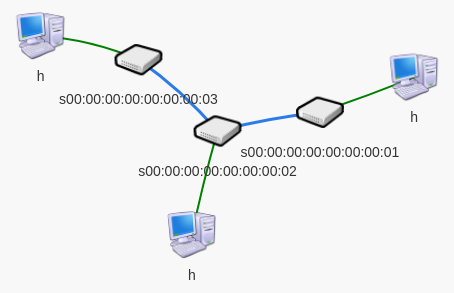
\includegraphics[width=0.8\textwidth]{images/flDoS}
	\caption{Denial of Service Floodlight Topology}
	\label{fig:images-flDoS}
\end{figure}

\subsubsection{SYN Flood}

Using the Wireshark packet analyzer tool. test est

\subsubsection{ICMP Flood}

\subsection{Distributed Denial of Service}

The Distributed Denial of Service topology was verified within the Floodlight
web server. Figure \ref{fig:images-flDDoS} displays the results of this, with
8 switches with 8 hosts each, and a final switch connected to the single target
server node.

\begin{figure}[H]
	\centering
	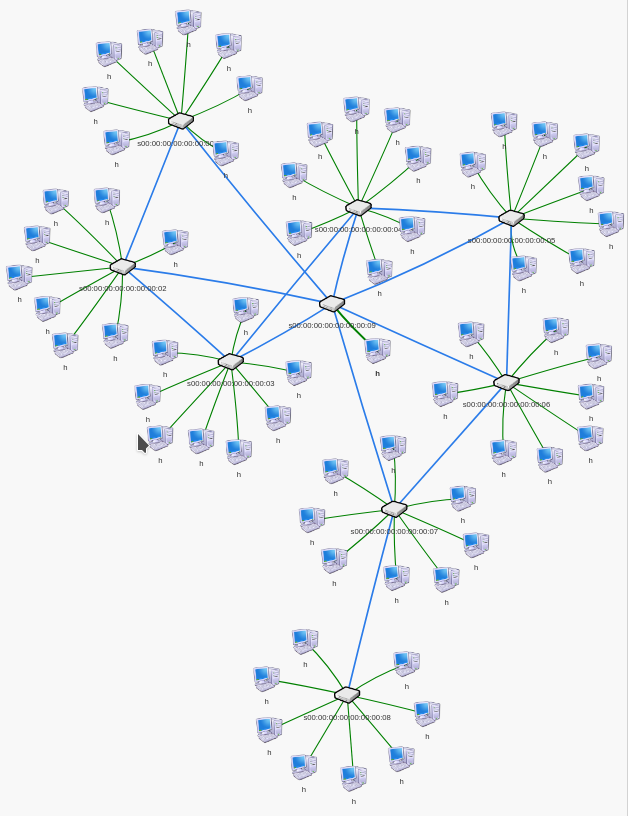
\includegraphics[width=0.8\textwidth]{images/flDDoS}
	\caption{Distributed Denial of Service Floodlight Topology}
	\label{fig:images-flDDoS}
\end{figure}

\subsubsection{SYN Flood}

\subsubsection{ICMP Flood}
